\chapter[Future Work]{Future Work} \label{appendix-future-work}
% \epigraph{All things are too small.}{Hadewijch of Brabant \cite{rothfeldAllThingsAre2024}}

\epigraph{[W]e have adhered to the late Thomas Schelling’s dictum that a model is finished not when nothing else can be added, but rather when nothing else can be taken away}{Rob Axtell \cite{axtellDynamicsFirmsData2024}}


% In  this chapter, we discuss potential extensions of our basic model. 
Our goal in this thesis has been to make a simple model that illustrates essential principles. % like the  the Alonzo model \cite{alonsoLocationLandUse1964}. 
We have sharply restricted our model  in order to focus on one process of significance, financialization, but we have designed the model to accommodate a range of extensions. In many cases, the natural extension is connecting this work, with other existing bodies of work or models.  In this chapter, we review what we have and then describe potential extensions in each area, along with several examples as well as hypotheses about what those extensions might fproduce. 

{\newpage\thispagestyle{empty}
\vspace{-1.5cm}
\begin{figure}
\vspace{-4.5cm}
\begin{adjustwidth}{-0.24\textwidth}{-0.2\textwidth}
\centering
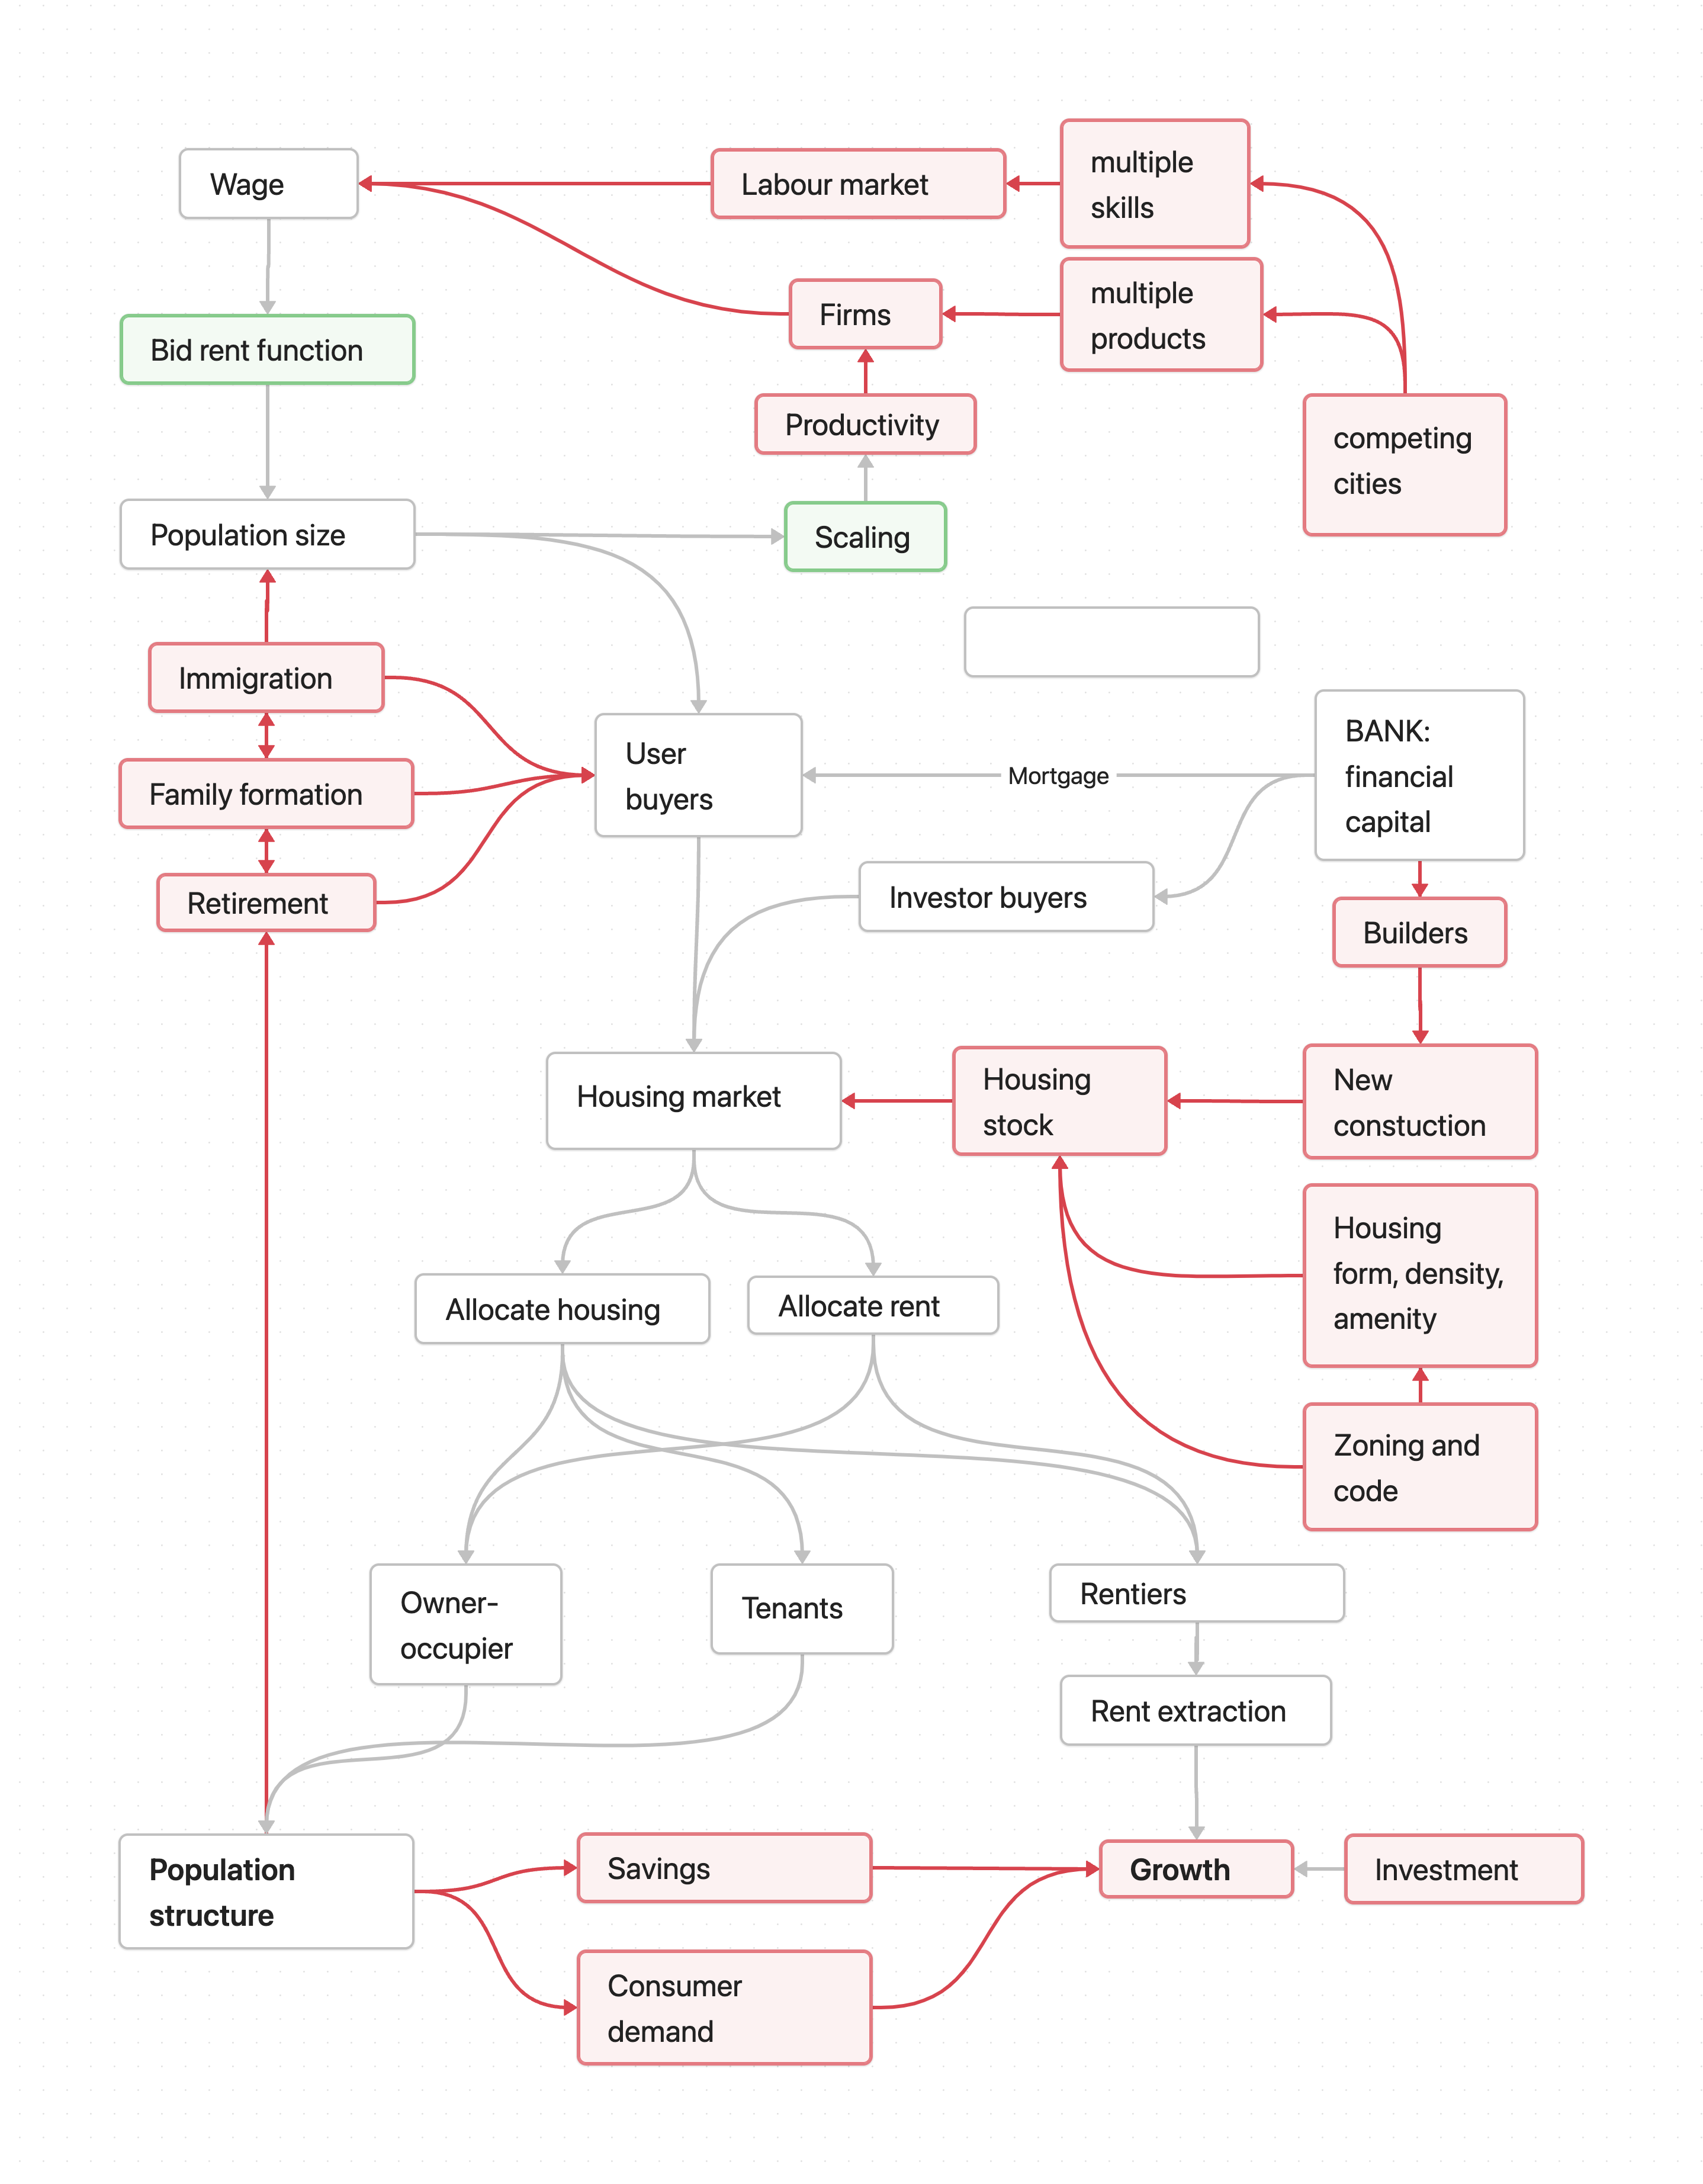
\includegraphics[scale=.22]{fig/extensions-logic.png}
\end{adjustwidth}
\caption{Extensions}
\label{fig-extensions-logic}
%\pagestyle{headings}
% \usetikzlibrary{positioning}
%\begin{tikzpicture}[remember picture,overlay,shift={(current page.north east)}] \node[anchor=north east,xshift=-1cm,yshift=-1cm]{\includegraphics[width=1cm]{example-image-a}};\end{tikzpicture}
\end{figure}}


% We have nevertheless designed the model to accommodate a range of extensions to explore questions that are theoretically or interesting or important for policy-makers.

% \section{Agents} % 2
% \section{Firms and institutions} % 3
% \section{Space} % 1
% \section{Boundary} % 4


% \section{What we have in this model}
In our current model, the urban firm %central place 
pays a uniform wage, $w$ to all employees, who have identical preferences and transportation costs where $w$ is an attribute of individual residents. Residents purchase or rent equal quantities of land at differing locations $l$ for identical housing.  There are transportation costs $T$ that depend on distance from the central place, so land close to the central place is more attractive than land farther from the central place.  The equilibrium concept is that a market with identical individuals with identical incomes and transportation costs will result in identical utilities. The result is that land rent must decline with distance from the central place to offset rising transportation cost. The size of the city is determined by population and lot size. Income and transportation costs will interact with lot size. The basic model can be initialized by matching the number of properties to the size of the population. % TODO check this, it is an old description.

We focus on extensions to this base model, and selected experiments that this model is well positioned to explore.  At the end of the chapter there is a brief discussion of directions for future work more broadly. Extensions may be to particular agents, whether residents, firms, investors, or land, or changes in the boundary, flow or connections with the larger system. Broader questions include the potential for understanding urban savings, or the effect of financialization as systems change that this work raises. % TODO Explain Figure~\ref{fig-extensions-logic}. % illustrates five general types of extension to the base model.  In each case, we introduce the class and give several examples. 

% Extensions to this base model can be organized by what part of the model they contribute to residents, firms, investors, land, or other institututions

\section{Variations in the model}

\subsection{Residents}

Residents, currently choose whether to work in the urban center or not, and receive identical wages. They differ in their available resources, the savings they begin/enter with. We can introduce more nuanced agent heterogeneity. They may have different incomes, skills, preferences, or transportation patterns. Much of the complexity of the model is in the financial decision making process, which can be further nuanced. Residents may also act as consumers as well as workers, creating  local consumer demand.

\subsubsection{Income differences}
% The basic model with Income differences: 

Introducing income differences may result in segregation by neighbourhood depending on income. Income can be purely earning, which requires a distribution of $w$ across agents. Income  might include investment income, which  a private rate of return and a distribution of assets across agents. 



%Buyers could consider neighbourhood pressures, demographic changes, changes in job location, desire for amenity etc. in their assessment of housing need. 

%With multiple bids agents can place the most competitive bids on those homes they prefer. If they have higher urgency they place strong bids on more homes. 

%Next buyers request a selection of homes to consider from a real estate agent. Those with higher need for housing look at more homes. The real estate agent offers a selection of homes based on the agent's requirements. A randomness parameter determines how many divergent houses are also considered. When the parameter is 1, the selection of homes is fully randomized, When it is 0, the agent sorts all available homes and offers those which fit the agents budget, space, and other requirements best.

\subsubsection{Savings, investment, and retirement behaviour}
The simple agent decision mechanism % population turnover 
in our model can be replaced with a more complex set of possibilities at the agent level. Sufficient investment income could lead individuals to locate in cheap properties at the edge of the city.  Income might also be invested in property affecting the quality of a unit. This would require incorporating unit quality in the attribute list for each property, and introducing a quality preference  in the attribute s of residents.

At retirement,  agents can be allowed to may choose between selling their home, renting it as an income property, or if there is sufficient amenity value for them, staying in the city. Implementing these choices complicates the agent decision and the resulting housing distribution, and requires few changes to the rest of the model. 

\subsubsection{Rental bidding process}
Just as with prices, there is an economically \gls{warranted rent} which may differ from the \gls{market rent}. Individuals make their investment decisions on their own expectations rents. the bidding process on rental properties is abstracted in the base model. Instead of modelling the process explicitly, we make the assumption that the warranted rent is the market rent, $\mathcal{R}_W = \mathcal{R}_M$." .. could implement an explicit rental market to model rental prices explicitly.

\subsubsection{Rent-own choice}
Introducing a rent-own choice means agents could make decisions about whether they wish to rent or buy. %This may result in the emergence of classes. 
Agents must have the capacity to borrow to purchase. Attributes of the agents and must now include  net assets,  an available interest rate, and a permissible mortgage.

We imagine a banker setting the mortgage rates and size. This can be done at the beginning of each period for each agent. 

With no income differential we expect equal utilities.

The basic model with earnings differences and a rent-own choice is likely to generate diverging classes as income differentials permit some to capture land rents from others. This situation is likely if borrowing costs decline with income and asset ownership.



\subsubsection{Population pressure} 

{\color{red}The first ?} is to move from a static population to a model with population pressure. % This appears on the left as a group of three new subroutines with connections to the elements of the model most directly affected. % Some links are left out to keep the figure readable. Examples of omitted links  are the channels through which  population affects labour supply and savings.  
Our basic model does not have a growing population. This conveniently allows us to isolate certain effects of financialization. Population pressure is one of the drivers of financialization because it amplifies speculative gains, however. As a result, one of the first extensions must be  to introduce population pressure.

There are two sources to consider: 
\begin{enumerate}
\item agglomeration effects that increase the wage and attract workers faster than the housing stock can respond. 

Worker agents from outside the city can always consider moving and accepting a job. 
% QUESTION - how to manage the flow of new agents?
%, or can make more from rents and moving away
\item immigration pressure.
\end{enumerate}
Under the  first, agglomeration economies drive population while under the second, population growth may drive agglomeration.

The growth of the housing stock will generally lag population growth, generating price effects and stock dynamics.
Agents will respond to increases in demand conditions. The perception that the market is tight or that prices are rising may lead to higher bids and reservation prices and shift results in favour of sellers.

If population exceeds the number of properties there are three margins to consider
	\begin{enumerate}
		\item The land supply can increase. There may be a conversion cost
		\item The land per-capita may decrease. This is not simple in a city with land-use regulations, zoning, and fixed capital in homes. A conversion process has to be defined
		\item A homeless population can emerge. 
	\end{enumerate}


\subsection{Forward looking agents}
There are reasons to expect the results obtained with  forward-looking agents to differ substantially from those obtained with a model featuring myopic agents.\footnote{For example, Lecca et al. *** \cite{LOST-Lecca-et-al-2013}  used a stylized computational macroeconomic model applicable to a regional context to demonstrate that the assumption of myopic vs forward-looking agents yields differences in the dynamics generated by a shock perturbing the initial steady state, even though the alternative paths lead to the same long-run equilibrium.} 


\subsection{Amenity}

There may be a band surrounding the city or persons who do not commute but enjoy urban consumption amenities. 
based on location etc
Appendix discucses ammenity in more detail.

\subsubsection{The consumer city}

% At the bottom of the figure we introduce a fourth 
Another class of intervention, consumer demand, is linked to the population structure and feeding back to growth. In the real world, much of the demand for what is produced in the city is local consumer demand.  Our model has assumed there is production only for a perfectly elastic export demand. Consumer needs are buried in the subsistence wage. 

A minimal extension would be to introduce a second sector representing local consumption demand. A share of locally generated income would support production for the city's population. The labour force would be split between the two sectors and both productivity and wages might differ across sectors. A more complex treatment would introduce a range of service, entertainment and retail producers. This might be done monopolistically competitive firms as in Dixit and Stiglitz \cite{AvinashK.Dixit1977MCaO}. Savings behaviour would become more complex with endogenous consumer demand. % and with as more complex population structure.


\subsection{Firms}

Firm behaviour might also be enriched. We have  developed the link between neoclassical growth theory and the literature on urban scaling \cite{bettencourtIntroductionUrbanScience2021} and  we then imposed the scaling result on our model.  We force the model to conform to the empirical data on the relationship between population and productivity. This amounts to black-boxing the entire production and labour demand sector as well as the construction and housing production sector. 
% The fifth block of extensions illustrated in Figure~\ref{fig-extensions-logic} would 
We might replace the simple, scaling-based transmission mechanism in the Alonso-Jacobs cycle with explicit firm and labour market behaviour. % This class of extensions is obviously linked to population structure.
This leads to consideration of firms that produce different products, some for export some for the local market, and to multiple types of labour.

\subsubsection{Making labour market and firm behaviour explicit}

We could also explicitly model labour markets and competing firms. Explicitly modelling labour markets with multiple firms is a natural way to specify the model more completely, see Appendix~\ref{appendix-future-work},  but it would require introducing ancillary assumptions and selecting among alternative models of agglomeration, and we preferred to focus on distributional and growth-affecting features of the system.

Firm behavour could be modelled explicitly. We incorporate agglomeration effects at the aggregate level using a Cobb Douglas production function. This allows us to focus on the results of agglomeration in the urban system, rather than specifying the system of firms that transmit the effect. 
There are a number of other ways to study the agglomeration process in more or less explicit ways. We could include several representative classes of firms. %There are also very large models. 
% This made sense because our focus  was on the housing market and the financial sector, but the model we have constructed will allow us to ``fill the black box'' with more complete models of the production and labour market to see how they compare to the empirical data. 
A  model could allow individual wages to be linked to the agglomeration of other workers - say engineers. we can imagine a city that has centres of agglomeration by profession or by complementarity. Depending on the production function, this should emerge endogenously. Such a  model could get very large. Axtell explicitly models all firms in the US market interacting according to simple rules \cite{axtellDynamicsFirmsData2024}. It would be interesting to study the effects of space and local firm structure and opportunity, with interacting firms and financialization in the land market. 

\subsubsection{Infrastructure costs}
The scaling literature also provides relationships between density and population and infrastructure cost and population that we can explore in the same way. In the scaling literature, these relationships are increasingly theorized in terms of network effects, which is consistent with the Jacobs analysis and the more recent neoclassical growth modeling.


\subsubsection{Unemployment and labour adjustment costs}

We could introduce unemployment and \glspl{labour adjustment cost} for firms. %***INTERESTING TO THINK ABOUT  when people would stop working with % falls to subsistence wage - too much rent, I guess they leave, they can always move somewhere
% in the agent model, employees are simply laid off and seek work, so there is unemployment, but there are not \glspl{labour adjustment cost} for firms.

% \subsubsection{Business cycles}
% How does this connect with a business cycle. e.g. driving it with price signals connects this with a whole body of work with e.g. the work of Fabrice Collard. 
% % http://fabcol.free.fr/publi.html - in particular 

\subsection{Investors}

Much of the richness of this model is in the specification of agent investment behaviour. 
 

\subsubsection{Investment fund modelling}
Agents may fund their retirement from savings, as well as returns on their home if they have one to sell. Savings may be invested in a pension fund, or in local property,  depending on expected risks and returns. In the real world, financial institution manages most pensions, investing in the market or in property.  This institutional structure might be handled by implementing a savings account for each agent. % We are not interested in the detailed investment behaviour for the financial sector.% either in the stock market, or in pensions.
% Institutional and individual investors can access debt. %
We could also consider a case where outside money can come under institutional management, not just local retirement savings. A parameter would control the inflow of additional money beyond local investment in the pension fund. 

\subsubsection{Transaction costs}
Transaction costs on the sale of property are omitted. They are actually large. We can easily add a term to  Equation~\ref{eqn:maximum-bid} to examine the effect of transaction costs on the distribution of wealth.


\subsubsection{Risk, speculation, and business cycles}

There are many areas to explore in terms of the dynamics of the model. Risk plays a role in property markets. For example in Canada, backing mortgages is the largest fiscal 
investment at the national level \cite{nemtinFinancializationHousingSocial2021}. It is also possible to model the effect of speculative over-investment as expectations rise and fall, and the effects of business cycles as forcing of price and other parameters with external input to examine the effects.


\subsection{Land}

We could also add nuance to the modelling of land and space. 

\subsubsection{Housing production}

Financialization is not expansion of the housing stock, it is transfer of ownership. It is a process orthogonal to development. 
We could also introduce a housing production sector. This appears on the right side of of the figure linked to the banking sector. It requires adding a dynamic housing stock. Either dirrectly in the equations or explicitly by modeling the actions of agents aquiring and developing land. % to subdivide and develop. 

% \subsection{Financialization vs expansion of the housing stock}



% - it can lead to efforts to extract more rents by displacing people to invest in a shift in built form.
There are a number of potential links with the development process.

\begin{figure}
\begin{center}
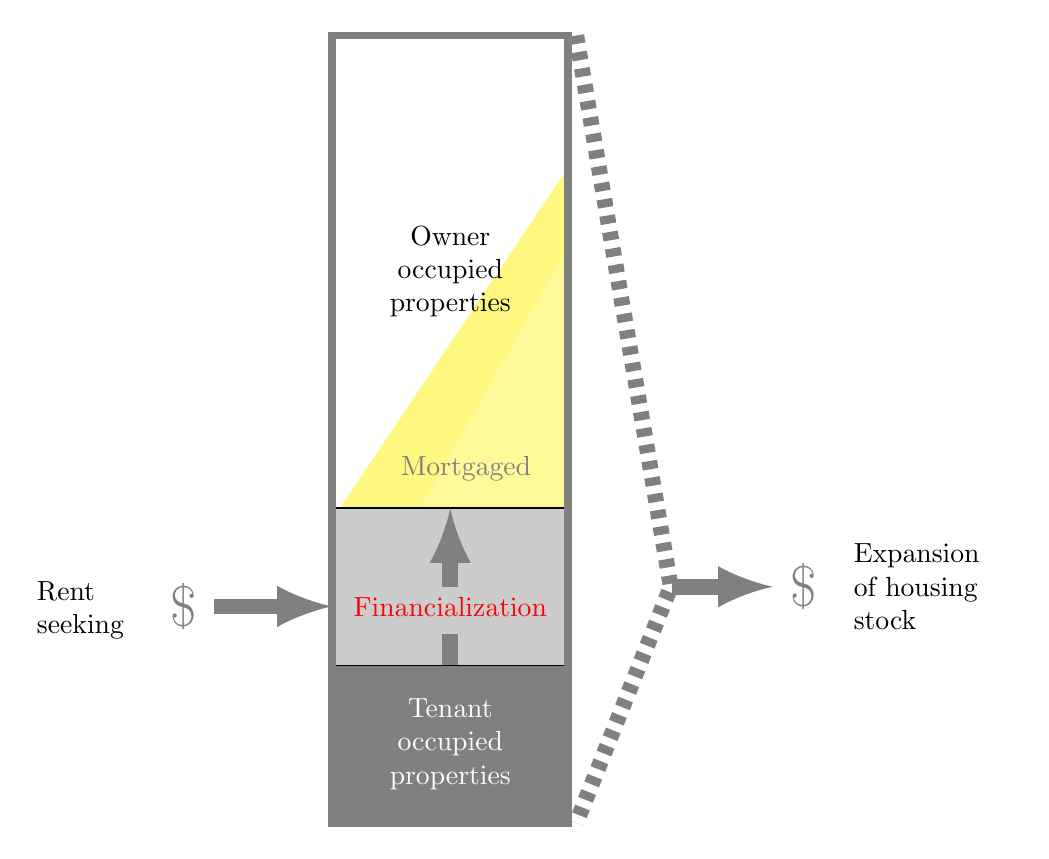
\begin{tikzpicture}{scale=.5}
\fill[yellow!50] (.1,4)--(3,4)--(3,8.33) --cycle;% MORTGAGE %Calculation. 80\%owner, so  8 above the tenant line. 2/3*8=5.333. 5.333+2=

\draw [fill=yellow!40] (0,2)--(3,2)--(3,7.33); --cycle;% MORTGAGE %Calculation. 80\%owner, so  8 above the tenant line. 2/3*8=5.333. 5.333+2=
\draw [fill=gray!40,opacity=1] (0,0) rectangle (3,4); %fiancialization   
\draw [fill=gray] (0,0) rectangle (3,2); %TENANT

\draw[line width= 1mm, black!50] (0,0) rectangle (3,10);

\node at (1.5,7)
    [text width=2.4cm, align=center]
    {\baselineskip=20pt Owner occupied properties};
\node at (1.7,4.5)
    [align=center, color=gray]
    {\baselineskip=20pt Mortgaged};
%\node at (2,3.3) [text width=2.4cm]  {\baselineskip=20pt Mortgaged};
\node at (1.5,1)
    [text width=2.4cm, align=center, white]
    {\baselineskip=20pt Tenant occupied properties};

%\draw [gray,line width=2mm](1.5,2)--(1.5,2.4) node[above, red]{Financialization}; 
\draw [gray,line width=2mm](1.5,2)--(1.5,2.4) node[above, red]{Financialization}; 
\draw [gray,-latex, line width=2mm](1.5,3)--(1.5,4);

\node at (-3,2.7)[ text width=1.5cm]{Rent seeking};
\draw [gray,line width=2mm,-latex](-1.5,2.75)node[left]{\huge$\$$}--(0,2.75);

%\node at (5.5,3)[text width=2cm]{Expansion of housing stock}; 
\draw [gray, dashed,line width=2mm,](3.1,10)--(4.3,3)--(3.1,0);

\draw [gray,line width=2mm,-latex](4.32,3)--(5.6,3)node[right]{\huge$\$$};
\node at (6.5,3)[right, text width=2cm]{Expansion of housing stock};
%\draw [gray,line width=2mm,-latex](6.5,3)--(7.5,3); 
\end{tikzpicture}


% OLDER JUST BOX LIKE ABOVE IMAGE WITHOUT FINANCIALIZATION, MONEY IN OR MONEY OUT
% \begin{figure}
% % 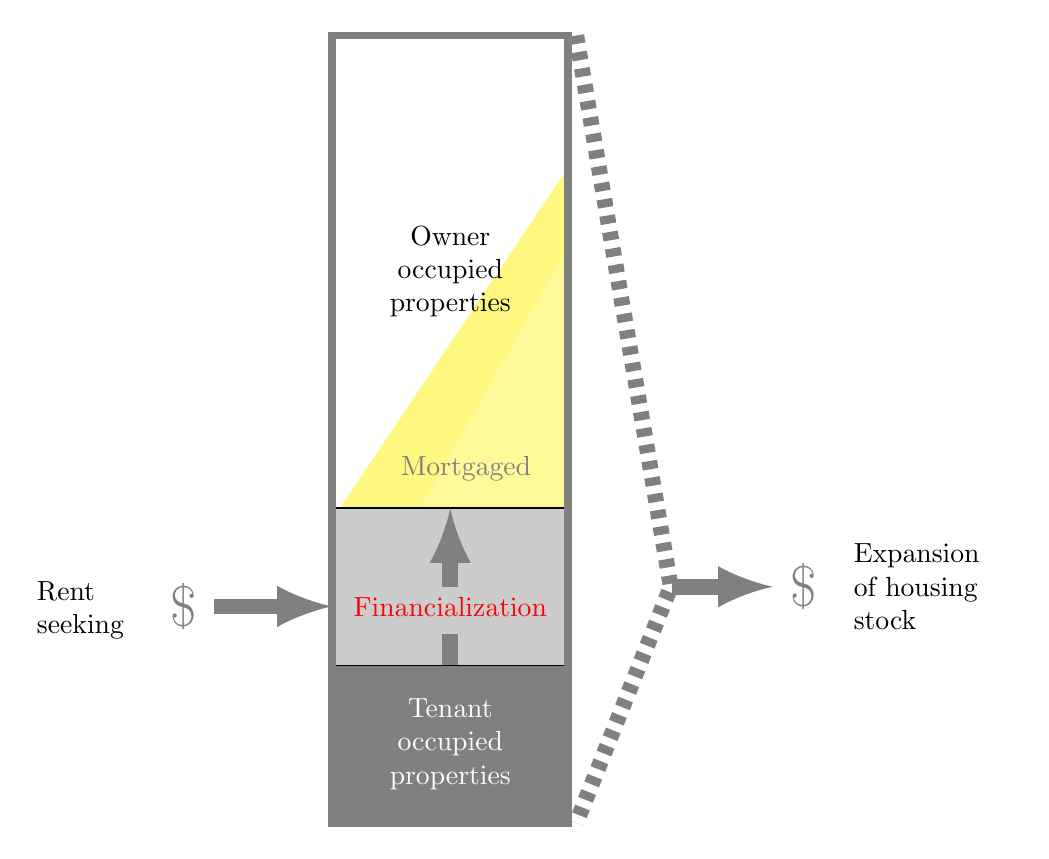
\begin{tikzpicture}{scale=.5}
\fill[yellow!50] (.1,4)--(3,4)--(3,8.33) --cycle;% MORTGAGE %Calculation. 80\%owner, so  8 above the tenant line. 2/3*8=5.333. 5.333+2=

\draw [fill=yellow!40] (0,2)--(3,2)--(3,7.33); --cycle;% MORTGAGE %Calculation. 80\%owner, so  8 above the tenant line. 2/3*8=5.333. 5.333+2=
\draw [fill=gray!40,opacity=1] (0,0) rectangle (3,4); %fiancialization   
\draw [fill=gray] (0,0) rectangle (3,2); %TENANT

\draw[line width= 1mm, black!50] (0,0) rectangle (3,10);

\node at (1.5,7)
    [text width=2.4cm, align=center]
    {\baselineskip=20pt Owner occupied properties};
\node at (1.7,4.5)
    [align=center, color=gray]
    {\baselineskip=20pt Mortgaged};
%\node at (2,3.3) [text width=2.4cm]  {\baselineskip=20pt Mortgaged};
\node at (1.5,1)
    [text width=2.4cm, align=center, white]
    {\baselineskip=20pt Tenant occupied properties};

%\draw [gray,line width=2mm](1.5,2)--(1.5,2.4) node[above, red]{Financialization}; 
\draw [gray,line width=2mm](1.5,2)--(1.5,2.4) node[above, red]{Financialization}; 
\draw [gray,-latex, line width=2mm](1.5,3)--(1.5,4);

\node at (-3,2.7)[ text width=1.5cm]{Rent seeking};
\draw [gray,line width=2mm,-latex](-1.5,2.75)node[left]{\huge$\$$}--(0,2.75);

%\node at (5.5,3)[text width=2cm]{Expansion of housing stock}; 
\draw [gray, dashed,line width=2mm,](3.1,10)--(4.3,3)--(3.1,0);

\draw [gray,line width=2mm,-latex](4.32,3)--(5.6,3)node[right]{\huge$\$$};
\node at (6.5,3)[right, text width=2cm]{Expansion of housing stock};
%\draw [gray,line width=2mm,-latex](6.5,3)--(7.5,3); 
\end{tikzpicture}


% OLDER JUST BOX LIKE ABOVE IMAGE WITHOUT FINANCIALIZATION, MONEY IN OR MONEY OUT
% \begin{figure}
% % 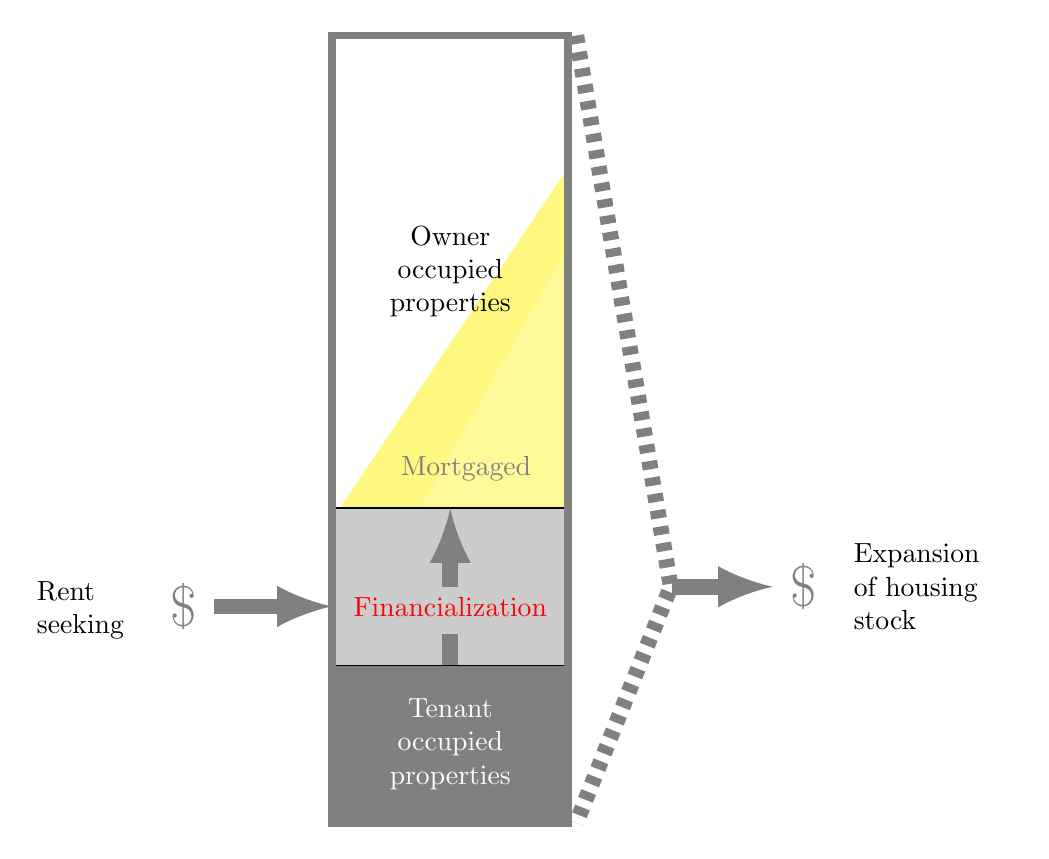
\begin{tikzpicture}{scale=.5}
\fill[yellow!50] (.1,4)--(3,4)--(3,8.33) --cycle;% MORTGAGE %Calculation. 80\%owner, so  8 above the tenant line. 2/3*8=5.333. 5.333+2=

\draw [fill=yellow!40] (0,2)--(3,2)--(3,7.33); --cycle;% MORTGAGE %Calculation. 80\%owner, so  8 above the tenant line. 2/3*8=5.333. 5.333+2=
\draw [fill=gray!40,opacity=1] (0,0) rectangle (3,4); %fiancialization   
\draw [fill=gray] (0,0) rectangle (3,2); %TENANT

\draw[line width= 1mm, black!50] (0,0) rectangle (3,10);

\node at (1.5,7)
    [text width=2.4cm, align=center]
    {\baselineskip=20pt Owner occupied properties};
\node at (1.7,4.5)
    [align=center, color=gray]
    {\baselineskip=20pt Mortgaged};
%\node at (2,3.3) [text width=2.4cm]  {\baselineskip=20pt Mortgaged};
\node at (1.5,1)
    [text width=2.4cm, align=center, white]
    {\baselineskip=20pt Tenant occupied properties};

%\draw [gray,line width=2mm](1.5,2)--(1.5,2.4) node[above, red]{Financialization}; 
\draw [gray,line width=2mm](1.5,2)--(1.5,2.4) node[above, red]{Financialization}; 
\draw [gray,-latex, line width=2mm](1.5,3)--(1.5,4);

\node at (-3,2.7)[ text width=1.5cm]{Rent seeking};
\draw [gray,line width=2mm,-latex](-1.5,2.75)node[left]{\huge$\$$}--(0,2.75);

%\node at (5.5,3)[text width=2cm]{Expansion of housing stock}; 
\draw [gray, dashed,line width=2mm,](3.1,10)--(4.3,3)--(3.1,0);

\draw [gray,line width=2mm,-latex](4.32,3)--(5.6,3)node[right]{\huge$\$$};
\node at (6.5,3)[right, text width=2cm]{Expansion of housing stock};
%\draw [gray,line width=2mm,-latex](6.5,3)--(7.5,3); 
\end{tikzpicture}


% OLDER JUST BOX LIKE ABOVE IMAGE WITHOUT FINANCIALIZATION, MONEY IN OR MONEY OUT
% \begin{figure}
% % \input{fig/financialization-expansion}
% \begin{center}
% \begin{tikzpicture}{scale=.5}
% \draw [fill=gray,] (0,0) rectangle (3,2); %TENANT
% \draw [fill=yellow!40] (0,2)--(3,2)--(3,7.33); --cycle;% MORTGAGE %Calculation. 80\%owner, so  8 above the tenant line. 2/3*8=5.333. 5.333+2=
% \draw[line width= 1mm, black!50] (0,0) rectangle (3,10);
% \node at (1.5,6)
%     [text width=2.4cm, align=center]
%     {\baselineskip=20pt\Large Owner occupied};
% \node at (2,3.3)
%     [text width=2.4cm]
%     {\baselineskip=20pt Mortgaged};
% \node at (1.5,1)
%     [text width=2.4cm, align=center, white]
%     {\baselineskip=20pt\Large Tenant occupied};
% % \caption{}
% \end{tikzpicture}
% \end{center}
% \caption{Housing tenure and mortgaged share.}
% \label{fig-mortgage-tenure}
% \end{figure}

% \begin{center}
% \begin{tikzpicture}{scale=.5}
% \draw [fill=gray,] (0,0) rectangle (3,2); %TENANT
% \draw [fill=yellow!40] (0,2)--(3,2)--(3,7.33); --cycle;% MORTGAGE %Calculation. 80\%owner, so  8 above the tenant line. 2/3*8=5.333. 5.333+2=
% \draw[line width= 1mm, black!50] (0,0) rectangle (3,10);
% \node at (1.5,6)
%     [text width=2.4cm, align=center]
%     {\baselineskip=20pt\Large Owner occupied};
% \node at (2,3.3)
%     [text width=2.4cm]
%     {\baselineskip=20pt Mortgaged};
% \node at (1.5,1)
%     [text width=2.4cm, align=center, white]
%     {\baselineskip=20pt\Large Tenant occupied};
% % \caption{}
% \end{tikzpicture}
% \end{center}
% \caption{Housing tenure and mortgaged share.}
% \label{fig-mortgage-tenure}
% \end{figure}

% \begin{center}
% \begin{tikzpicture}{scale=.5}
% \draw [fill=gray,] (0,0) rectangle (3,2); %TENANT
% \draw [fill=yellow!40] (0,2)--(3,2)--(3,7.33); --cycle;% MORTGAGE %Calculation. 80\%owner, so  8 above the tenant line. 2/3*8=5.333. 5.333+2=
% \draw[line width= 1mm, black!50] (0,0) rectangle (3,10);
% \node at (1.5,6)
%     [text width=2.4cm, align=center]
%     {\baselineskip=20pt\Large Owner occupied};
% \node at (2,3.3)
%     [text width=2.4cm]
%     {\baselineskip=20pt Mortgaged};
% \node at (1.5,1)
%     [text width=2.4cm, align=center, white]
%     {\baselineskip=20pt\Large Tenant occupied};
% % \caption{}
% \end{tikzpicture}
% \end{center}
% \caption{Housing tenure and mortgaged share.}
% \label{fig-mortgage-tenure}
% \end{figure}

\end{center}
\caption{Financialization expands investor ownership, but does not in expand the housing stock. Yellow represents privately owned homes for which ownership is partially held by mortgage lenders.}
\label{fig-financialization-expansion}
\end{figure}





\subsubsection{Density, housing form, and neighbourhood amenity}
Separable from production, it is possible, is to introduce variation of housing form,  density and amenity.  Many questions about who gets what housing arise at this point. 
% Consider adding density, to look at how it interacts with agglomeration effects.

Much of what is interesting in a city is the rich variety of housing forms and neighbourhoods and the varied populations that occupy them. Our model has a single form of housing and an undifferentiated populations, allowing us to differentiate the housing system in specific ways and study the interactions between the built world and the population.

Variable density is achieved by allowing stacking of housing units. Results for this model are not known. This introduces a step change in housing form, and emphasizes unit size. Variable lot size is achieved by making lot size a choice variable for households, in which case we will get a trade off between transportation cost and lot size and distance. Results for this model are known. Density falls with distance from the centre. 


\subsubsection{Distribution of rents}
Rents go to landowners, with a share taken for maintenance and taxes.
Rents may also be taxed, could be shared between multiple owners, etc.
 %\note{REPHRASE? rent is  extracted from the coalition of capital and workers.} % Rents may also be taxed, could be shared between multiple owners, etc. 
%The rents are captured by landowners.  The capture of rents by landowners is common buy not necessary. 
In principle the gains from urban productivity and amenity can be allocated as social wealth through shared ownership, as is often done on a small scale with cooperatives and land trusts, distributed to all citizens through something like a social wealth fund, or captured in taxes or fees as Henry George suggested. 
%The rents would otherwise go to labour and capital.

\subsubsection{Taxes and productivity} % municipal government, public goods, and productivity}
This is a major issue with considerable development in the economics literature. Property taxes reduce the net locational value that flows to an individual owner but provides services and wages that make the city attractive. 
% TODO (create a regime where particular groups have an advantage)
Localized tax advantages can move a share of financialised investment into private consolidation of land, 
including the structure of taxes for investment properties, institutional investors, individuals, etc.

Just as finacialization may extract resources that would otherwise be invested in increasing human capital, consumption or productivity, reducing productivity. Taxes could either be extracted or reinvested. There is some evidence taxes can increase productivity through infrastructure, education, public spaces, recruiting employers, and direct investment, etc. Re-distributive programs are expected to have direct distributional effects. These could be explored through additional linkages in the model.


\subsubsection{Regulation and zoning}
We can ask what would be the effect of a hard zoning boundary and what would be the effect of suddenly relaxing it. We could explore the effect of speeding the rate of conversions from one size  home to another, or of locating high density pocket on a transportation route. Many significant urban policy questions could be examined with a limited amount of additional programming. 
% Zoning restrictions and building codes are related.

\subsubsection{Locational preferences}
Locational preferences may result in segregation by neighbourhood depending on preferences. One version would be include distance to the edge of the city as an amenity in resident's utility function. Another would be to locate amenities within the city. These would lead to higher prices near amenities. A third variant would be to have earning depend on location. If there were several locations a polycentric city would emerge.


\subsubsection{Transportation costs} % and the evolution of the city} \label{section-transportation}

Another spatial feature that can be greatly filled in in the model, is the transportaiton cost. Wage and transportation cost determine the radius of the circular city, which determines the size of the labour force which affects urban productivity. The cost of travel is therefore an important variable in the development of urban productivity. 

the transportation cost/distance relationship appears to be non-linear in many cases. While the linear model connects with the established literature, we likely want to explore the implications of more empirically grounded curve (e.g. \cite{bertaudSpatialDistributionPopulation2003}).




Varied transportation costs will result in segregation by neighbourhood depending on income and transportation costs. Experiments include cars for those who can afford them overlapping with transit. % Diagnostics include change in total transportation cost and differential welfare effects.
Urban transportation is primarily a municipal responsibility and major component of the municipal budget. Private transportation costs can be affected by municipal planning, construction, and regulation. Transportation costs are therefore a policy variable.  A decline in private transport costs results in an increase in the social surplus generated by the city. One feature of interest when we examine financialization is whether the surplus generate by investment in the transportation system goes to residents, firm owners, the public sector or to financial capital. 
% The problem is to determine to whom it goes. 

% Transportation costs are not likely to be affected appreciably nor quickly by the financialization of housing, so we have implemented a simple, uniform transport cost in our basic model. 


The theory implies that transportation improvements that reduce the cost of travelling to work should  affect affect rents, but effect may spillover or leakage  onto wages  at the centre or allow for city expansion at the edge.   
To see how, consider an expenditure that decreases transport costs.  A simple version of the urban economic theory  that underlies our  model can be summarized by the equation that for each household, rent plus transportation costs add up to a constant \cite{sootTransportationCostsUrban1974c}.\footnote{The formula assumes that access to work is the only goal of transportation for households, that there is a single mode of transport available and that households are able to minimize the sum of rent and transport costs. None of these are strictly true, and cannot relied on for a fine-grained analysis of the city, but are very convenient for our purposes.} % We have however, given some thought to how to introduce transportation costs into a model if it is applied to planning issues. 
The degree of spillover will be very sensitive to the relative elasticities of demand and supply  for labour, land, consumption, and local densities. These leakages will reduce the amount of the social gain captured as land rent. Without building in elasticities we % We  have not built the elasticities into our model so we 
cannot make predictions for specific cities or situations. %We know, however, that who gets the rents in determined by the degree of financial ownership of  the housing stock. This we can and will explore. 

We can derive qualitative results. For example, if reducing transportation costs make more land economically available for city expansion, increased supply should reduce land rents at the centre and increase labour supply, reduce wages and increase output.  But what if land is not cheap at the edge of the city and density cannot adjust? The city cannot grow. The decrease in transportation cost will increase the effective wage, and will have a bigger effect the farther a household resides from the centre. ($\partial{\omega-cd}{c}>0$) and rents in the periphery will rise. With a fixed population they should therefore fall at the centre. But the locational rent at the centre is equal to the wage premium, so there should also be downward pressure on the wage, but not labour costs, making labour more available for the same wage premium. The effect on rents land rents may vary. If transportation cost keeps falling and lots of land is available, then you don't get strong increases in land prices. If there are strong differentials, that gives the class result in the city, but doesn't tell you how it would affect it. 


\subsection{Broader questions for future work}

The simple case we examine will allows us to focus on the general, and neglected, distributional features of this class of models, however the simple circular city can be extended to to produce other forms, including polycentric cities and hierarchies of cities at the cost of additional computational complexity. There are other important questions to explore. The city is one city among others, how does it connect with the larger system of cities.

\subsubsection{The system of cities}
Modern cities are not lonely and autarkic  beasts wandering their own exclusive territory. % and unconnected to others of the species. 
Each city is one in a global system of cities that compete with and complement each other. Information, capital and even labour flows between cities are large. Henderson Abdel-Rahman \cite{Henderson1972Sizes}, Abdel-Rahman \cite{abdel-rahmanAgglomerationEconomiesTypes1990}, Fujita \cite{fujitaMonopolisticCompetitionModel1988}, Fujita, Krugman, and Venables \cite{fujitaSpatialEconomyCities1999}, and Fujita and Thiess \cite{fujitaEconomicsAgglomeration1996} among others provide models for expanding the model in this direction. 

% Linked to the labour market and production system is the possibility of introducing competing cities. 

% Lots of variations are possible, for instance 2 cities with immigration, differentiated labour, products, market power, neighbourhood effects. % (see extensions map/typology) multiple cities, linear cities, of the system, including the relations with other cities, and larger flows


\subsubsection{Urban savings}
% TODO THIS IS A CONTRIBUTION, BUT ALSO A DISCUSSION OF ONE WAY THIS WORK COULD BE EXTENDED, MIXED WITH A BIT OF MODEL DESCRIPTION

Conventional growth models specify a savings/investment mechanism at the national level. To our knowledge, this has not been done for the city level. We require  savings at two levels. First, since we want to incorporate  households home ownership and a relationship to the financial sector through mortgages, We specify a savings rate out of the spending we have isolated in the `subsistence wage' This means that both urban and rural workers accumulate savings, that savings are age-dependent, making the size of mortgage available also age dependent. 
Homeowners in addition have equity $E=P-M$ in their homes. % ({\color{red}Should newcomers also have equity? or is it built into the savings. Clarify this.} 

A second level of saving is the  investment in capital out of the city surplus. %Even raising this question puts us into terra incognita. 
There are many  channels through which surplus flows into productive investment in the urban contest. One is through public investment in infrastructure. We have discussed how falling transportation costs increase surplus generation. Investments like this are made slowly and take effect over time periods much longer than our model is concerned with.  We can set a property tax rate   that we will assume is sufficient to maintain the stock of infrastructure.

Public and private investment in human capital is largely urban as well, but as with infrastructure, investment and response take effect over time periods much longer than our model is concerned with. Private sector innovation in technology, marketing, or products draws on local saving less but still significantly on local savings. We have little in the way of theory or empirical research on this channel. Lags between investment and any rise in the urban wage premium are almost certainly long and variable. 

We deal with this issue by linking local capital ownership with the scale factor. It is known that local ownership is associated with local investment. We will assume that local capital ownership, which consists in part of local ownership of the housing stock, can be proxied by homeowner equity as a share of local. 

\subsubsection{Financialization as system change} \label{section-system}
We established that, at least in theory, financial institutions and the wealthy are likely to own increasing shares of the housing stock. The theoretical conclusions is consistent with what has already happened in the Canadian Housing market. Recent data from Statistics Canada \cite{fontaineResidentialRealEstate2023} suggests people who own more than one property in Ontario make up more than 25\% of buyers in the province. (The proportion of investors among owners varied from 20.2\% in Ontario to 31.5\% in Nova Scotia.)
Just under one in five properties overall was used as an investment.
In Ontario 41.9\% of condominium apartments are investment properties \cite{statisticscanadaBuyRentHousing2022}.

The immediate social implications are fairly obvious. As Statistics Canada points out, these trends might limit the number of properties available to buyers who intend to use it as a primary place of residence  \cite{fontaineResidentialRealEstate2023}. Statistics Canada reports that latest census release, two-thirds of Canadians owned a home in 2021, down from a peak of 69 per cent a decade earlier. The decline is was higher for younger members of the population. 

When the homeownership rate goes down, the rental rate goes up. The 2021 Canadian Housing Survey reported that the number of renter households increased  at over twice the pace of owner households, pushing down the homeownership rate in Canada. If the trends continue, Urban Canada will gradually change from a society dominated by homeowners to a predominantly tenant society. Since wealthier buyers are advantaged in the market, the younger and poorer parts of the community will be increasingly excluded from ownership. Financialization will increase income and asset inequality in cities.

Combined with rising housing prices the effect will be to squeeze lower-wage households closer to what we have termed to subsistence level and make it harder for low-wage workers to live in the city. The city requires low-wage workers for many of the services, so labour shortages are a possibility. Labour shortages will squeeze some activities out of the city and are likely to reduce productivity. Labour shortages may push up wages, but in rental markets, landlords can capture much of any increase in wages. 

The incentive structure in our model was derived purely from the point of view of an individual investor. Examination shows that investment incentives favour the wealthy and institutional buyers, but that does not necessarily imply that the process of financialization will drive social transformations. % Individual choices are at most  a link in the chain.
Modelling  allows us to ask %identify 
which parameters are most influential. 
A question that is especially important is whether the process of financialization and tenentization our micro model suggests is reversible:  high levels of home ownership we have seen throughout the 20$^{th}$ century. %, as Purdy 

\section{Variations in method and validation}

% In the above sections, we've detailed several promising directions for future work using this base model. %, as well as ways to expand the model, and connect with other work. 
In addition to extending the model, there are variations in what we do with the model or how we validate it. We may do more experiments, better characterize the model, or integrate it more systematically with data, or use it with different audiences. %, as well as to combine experiments to explore phenomena. 


% \begin{enumerate}
%     \item extension to the model, 
%     \item the integration of additional data, 
%     \item furthur analysis, experimentation, and exploration.
% \end{enumerate}



\subsection{Experimentation}
\subsubsection{Initial state and parameter values}
Basic experiments has all homes owner occupied to start. Other initial tenure mixtures are easily modelled. WHY WE MIGHT WANT TO

The basic model can be initialized by matching the number of properties to the size of the population. 

In the simplest version, firms concentrate at the city centre. Workers are spread over space and pay transportation costs to commute.

The size of the city is determined by population and lot size. Income and transportation costs will interact with lot size. 


\subsubsection{Sensitivity analysis}

mapping of regimes
More comprehensive analysis includes
- sensitivity analysis
- statistical issues
- non linear dynamics, hysteresis, and resilience. % Nonlinear dynamics, resilience, and hystersis
These models may exhibit irreversibilities in variables such as distribution, homelessness, city form, and class structure. 
A straightforward strategy for examining the system resilience is to shock a model (experiment) and then see if diagnostic variables recover. % (This needs more precise expression.) % While there  are many variations on the basic urban model and many potential experiments with each model there are only a few of immediate interest if the goal is to test the ``resilience'' of equilibria.
A first step would be shocks adding - cyclic behavour to price, shocks  to the labour market.



including with more comprehensive sensitivity and xx analysis, and analysis of the nonlinear dynamics, hysteresis and resilience properties, 

\subsubsection{Combinatorial experiments}

% Extensions from this basic model can go in several directions. We treat three categories of extension to this model:
% There are many more possible models than this, and these extensions combine. 
These extensions combine. Models are by nature combinatoric: every added element involves making a choice among alternative assumptions and implementations. Each extension is potentially as complex as the core model, and each introduces additional assumptions.  A model incorporating in binary choices is one of an implicit family of $2^n$ alternative models. 
They also describe a particular logic, which may be explored or studied in any particular region or context, drawing on local data and estimated parameter values. The context will also suggest, in many cases theoretical extensions, or particular questions.


% There are also combinations all of these above, for instance:


% The basic model with earnings differences and variable lot size: 
% The wealthy would likely larger homes and lots farther form the centre

% This model would likely produce some interesting spatial patterns, especially if couples with the possibility of secondary central places.

% The basic model with earnings (Y) differences, constant lot size and variable density: This model should produce some interesting spatial patterns, especially if coupled with the possibility of secondary central places.



\subsubsection{Lags and adjustment processes}
The details of the adjustment process and the system lags are selected primarily for convenience in simulations. Real-time lags are important and complex, we explore some sensitivity results, but can explore more. 

We model a fairly short lag although in reality lags are long and variable. 




% In practice these are combinatoric, each experiment may be combined with many others. We don't go into details on rich set of ways this model may be connected or be a part in the models of others (DEREK'S), for instance replacing the stylized model of transportation costs with rich empirical model of a transportation system as a dynamic system like that in the work of XX, or replace the representative urban firm model with an evolving system of agent based firms \cite{axtellDynamicsFirmsData2024}. 



\subsection{Data}
n each case, to make claims about the world, whether predictive or explanatory, that go beyond illustration and 
theoretical exposition, requires engagement with data.  %Also possibl eot change the purpose of modelling

 or other explorations with the model. We can also bring in new data. using it for something related to practice - as a boundary object for social learning.


There is also potential for this work to expand to engage with other fields and be used in practice.

\subsection{Audiences}
ABMs can be run multiple times to produce distributions of expected outcomes, which makes them valuable in planning exercises.
We divide experiments into two categories 1. more comprehensive analysis of of the model and 2 experiments to answer new questions

as boundary object, etc.
USE WITH PEOPLE IN SCENARIOS ETC
Use in scenario exercises


\section{Summary}


Incorporating these extensions, we can explore relatively fine-grained effects of financialization. The examples that follow  illustrate   ways the model can be extended and suggest further hypotheses that we  would like to test using our model. We would argue that it's likely none of them would change our qualitative results greatly, however each would deepen our understanding of mechanisms and of the detailed impacts. 

We divide extensions two broad categories of extensions. Changes to this model, keeping the same basic agents and equilibrium assumptions, and changes to that basic structure, for instance to introduce a multi-agent model of firm behaviour. % In our agent based model, in which every lot is  addressable, it is simple to 
For instance, we might introduce zoning boundaries, local amenities, different densities or housing qualities and homes of different sizes. % Hundreds of experiments are possible exploiting  the extensibility we have carefully conserved.  
% Likely few of the possible extensions would affect our qualitative results. 
In addition to changing the structure of the model, we can also bringing in data, characterising the model engaging with statistical issues including non-linear analysis and hysteresis, integrating data or exploring policy alternatives.



